%% 
%% Copyright 2026 Elsevier Ltd
%% 
%% This file is part of the 'Elsarticle Bundle'.
%% ---------------------------------------------
%% 
%% It may be distributed under the conditions of the LaTeX Project Public
%% License, either version 1.2 of this license or (at your option) any
%% later version.  The latest version of this license is in
%%    http://www.latex-project.org/lppl.txt
%% and version 1.2 or later is part of all distributions of LaTeX
%% version 1999/12/01 or later.
%% 
%% The list of all files belonging to the 'Elsarticle Bundle' is
%% given in the file `manifest.txt'.
%% 

%% Template article for Elsevier's document class `elsarticle'
%% with numbered style bibliographic references
%% SP 2008/03/01

\documentclass[preprint,12pt, a4paper]{elsarticle}

%% Use the option review to obtain double line spacing
%% \documentclass[authoryear,preprint,review,12pt]{elsarticle}

%% For including figures, graphicx.sty has been loaded in
%% elsarticle.cls. If you prefer to use the old commands
%% please give \usepackage{epsfig}

%% The amssymb package provides various useful mathematical symbols
\usepackage{amssymb}
\usepackage{hyperref}
\usepackage{url}
\setlength{\parindent}{0pt}
\setlength{\parskip}{4pt}
%% The amsthm package provides extended theorem environments
%% \usepackage{amsthm}

%% The lineno packages adds line numbers. Start line numbering with
%% \begin{linenumbers}, end it with \end{linenumbers}. Or switch it on
%% for the whole article with \linenumbers.
%\usepackage{lineno}

\journal{SoftwareX}

\begin{document}
\renewcommand{\labelenumii}{\arabic{enumi}.\arabic{enumii}}

\begin{frontmatter}

\title{pynhts: survey-weight-aware Python access to the US National Household Travel Survey}

\author[affa]{Seyed Saber Naseralavi\corref{cor1}}
\ead{saber\_naseralavi@uk.ac.ir}
\author[affb]{Akram Mazaheri}
\ead{akram.mazaheri.010@gmail.com}
\cortext[cor1]{Corresponding author}

\address[affa]{Department of Civil Engineering, Shahid Bahonar University of Kerman, Kerman 7616914111, Iran}
\address[affb]{Department of Civil and Environmental Engineering, Tarbiat Modares University, Tehran 1411944961, Iran}

\begin{abstract}
The US National Household Travel Survey (NHTS) is the main public source of US household travel data, and four waves (2001, 2009, 2017 and 2022) are freely available. Using them correctly is harder than it looks: weights and variance designs differ by wave, the same code can mean different things in different waves, skipped questions are stored as numbers, and trip weights give annual rather than daily totals. These details are rarely stated in papers, so published results are difficult to reproduce or to compare. pynhts is an open-source Python library that downloads and verifies the official files, converts them to typed Parquet, joins the four tables without silent errors, and computes estimates with the variance method of each wave (jackknife replicate weights for 2001, 2009 and 2017; Taylor linearisation for 2022). It adds validated crosswalks between waves, guards for top-coded and non-answer values, and a study module that turns a written research statement into an analysis file with a sample-flow table. Validation is part of the package: 142 of 175 figures printed in official reports reproduce completely, Taylor-series errors agree with R to 1e-9, and 21 published studies were rebuilt and 1,096 printed numbers graded. The rebuilding recovered unstated rules, such as the base of a percentage and the definition of a weekend, that move published values by several per cent. The package is young and has no external users yet; its contribution is a tested, documented way to state and check the assumptions of NHTS analyses.
\end{abstract}

\begin{keyword}
National Household Travel Survey \sep travel survey \sep replicate weights \sep survey statistics \sep reproducibility \sep Python
\end{keyword}

\end{frontmatter}

%\linenumbers

\section*{Required Metadata}

\section*{Current code version}

\begin{table}[!h]
\begin{tabular}{|l|p{6.5cm}|p{6.5cm}|}
\hline
\textbf{Nr.} & \textbf{Code metadata description} & \textbf{Please fill in this column} \\
\hline
C1 & Current code version & v0.8.1 \\
\hline
C2 & Permanent GitHub link to code/repository used for this code version & \url{https://github.com/sabernaseralavi-60/pynhts} \\
\hline
C3 & Legal Code License & BSD 3-Clause License \\
\hline
C4 & Code versioning system used & git \\
\hline
C5 & Software code languages, tools, and services used & Python 3; NumPy, pandas, PyArrow, pooch, PyYAML; optional: matplotlib, PyTorch \\
\hline
C6 & Compilation requirements, operating environments \& dependencies & Python 3.10 or newer on Linux, Windows or macOS (continuous integration on Linux and Windows); about 0.4 GB of Parquet per wave and 1.8 GB of raw CSV for 2017, which can be deleted after conversion \\
\hline
C7 & If available Link to developer documentation/manual & \url{https://github.com/sabernaseralavi-60/pynhts/tree/main/docs} \\
\hline
C8 & Support email for questions & saber\_naseralavi@uk.ac.ir \\
\hline
\end{tabular}
\caption{Code metadata (mandatory)}
\label{tab:meta}
\end{table}

\textbf{Main text}\\

\begin{enumerate}

\item \textbf{Motivation and significance}\label{sec:motivation}\\

The National Household Travel Survey (NHTS), sponsored by the US Federal Highway Administration (FHWA), is the main public source of information on how US households travel: who makes trips, by which mode, for which purpose and over what distance \cite{mcguckin}. Public-use files exist for 2001, 2009, 2017 and 2022, each with four linked tables (households, persons, trips, vehicles), sampling weights and, for three waves, replicate weights. The files are used for many topics. Recent examples are access to health care \cite{labban}, the mobility of older adults across waves \cite{buehler,akinlotan,lidbe}, taxi and ridehailing use \cite{conway,rafiq}, ridesharing and vehicle ownership \cite{zhang}, alternative fuel vehicles \cite{li}, vehicle miles travelled \cite{alberini,wu}, active travel \cite{yang} and online shopping \cite{zhou}.

Working with the files is less simple than the number of such studies suggests. Several authors have shown how the survey itself shapes results: respondents who agree to be contacted again differ from those who do not \cite{wang}, proxy responses contain more rounded departure and arrival times \cite{yoshikawa}, and a representation measure built from sampling weights found under-representation of vulnerable traveller groups in 43 US household travel surveys, the 2017 NHTS among them \cite{esekhaigbe}. Beyond the properties of the survey, correct use requires work that every project repeats and that is easy to get wrong. A skipped question is stored as the number -1, so the mean of the 2009 vehicle miles driven (VMT\_MILE) is 5.36 instead of 9.72 and its total is 7\,\% low. The same code means different things in different waves: transport mode ``01'' is a car in 2009, where it is 44\,\% of trips, and walking in 2017, where it is 10.5\,\%. Trip weights add up to annual, not daily, totals; the 2001 file contains children aged 0--4 and the others do not; ages and vehicle ages are top-coded; and 2022 uses a different variance design from the earlier waves. Such mistakes change estimates and, more often, understate their uncertainty. Papers rarely state the rules they applied, which makes their numbers hard to reproduce.

This matters beyond one survey. Calls for reproducible transportation research ask for open code and documented methods \cite{zheng,wood}, and name insufficient methodological detail and the lack of code sharing among the barriers \cite{wood}; agent-based travel-demand research is rarely replicable when it rests on proprietary data and tools \cite{horl}. In the wider research-software community, the FAIR principles have been adapted to software \cite{lamprecht,barker} and principles for software citation have been proposed \cite{smith}. pynhts follows them in practice: every release is archived with a persistent identifier and a machine-readable citation file.

pynhts addresses these problems in one Python package. It (i) fetches and verifies the official files and exposes them as typed tables that cannot be merged wrongly, (ii) computes every estimate with the variance method of its wave, (iii) maps codes between waves only where the meaning is shown to be the same, (iv) requires the analyst to state sample rules, missing-value policy and weighting, and (v) ships its own validation against published numbers. Scientifically, the contribution is not a new estimator but a way to make the assumptions of an NHTS analysis explicit, testable and reusable. A user installs the package, downloads a wave with one command, loads it lazily, and asks for weighted statistics, rates, harmonised categories or a complete study (Section~\ref{sec:examples}). Results carry the wave, weight, variance design and unit, so a table footnote can be written from the result itself.

Related work. The R package summarizeNHTS \cite{summarize} downloads and summarises NHTS data, and the R survey package \cite{lumley} offers general replicate-weight and Taylor-series analysis that users can apply to NHTS data after setting up the design themselves. The Python package samplics \cite{samplics} covers complex-sample estimation in general but does not know the NHTS files, codes or weights. A search of GitHub and PyPI on 22 October 2026 (queries ``NHTS python'' and ``national household travel survey'', and the package names nhts, nhts-py and summarizenhts) found analysis scripts for single projects and no other general Python package for NHTS access. The variance estimators follow the standard replicate-weight theory \cite{wolter} and the weighting report of the 2017 survey \cite{weighting}.

\item \textbf{Software description}\label{sec:architecture}\\

\begin{enumerate}
\item \textbf{Software architecture.} pynhts is organised in layers (Fig.~\ref{fig:arch}). The input and statistics layers handle the data; the harmonisation and analysis layers help the analyst to ask correct questions; the validation layer checks the result against published numbers.

\begin{figure}[!ht]
\centering
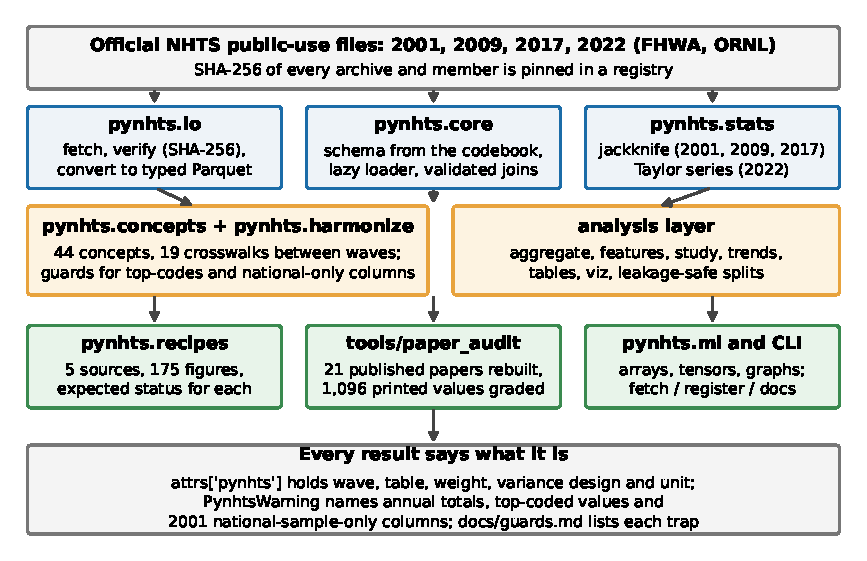
\includegraphics[width=0.92\textwidth]{figures/fig1_architecture.pdf}
\caption{Architecture of pynhts. Blue: data access and statistics; amber: harmonisation and analysis; green: validation and bridges. Every result frame records how it was computed.}
\label{fig:arch}
\end{figure}

pynhts.io keeps a registry with the SHA-256 hash of every official archive and member, downloads with pooch, and writes Parquet deterministically. The data server answers HTTP 200 with an HTML page for files that do not exist, so content type and size are checked. pynhts.core derives a typed schema from the codebook (all 3,807 coded values of 2017 and all 2,639 of 2022 reproduce the printed frequencies) and loads columns lazily, joining each requested column from the table that owns it through a validated many-to-one join. The skip code is converted to a missing value in numeric columns by default, and non-answer codes are masked on request.

pynhts.stats implements the stratified jackknife of the 2017 weighting design. With 14 variance strata of 7 units, the variance of an estimate is 6/7 times the sum over the 98 replicates of the squared deviation of the replicate estimate from the full estimate, and the margin of error (MOE) is the t quantile with 98 degrees of freedom times the standard error \cite{wolter,weighting}:

\begin{equation}
\hat V(\hat\theta)=\frac{6}{7}\sum_{r=1}^{98}\bigl(\hat\theta_r-\hat\theta\bigr)^{2},\qquad \mathrm{MOE}=t_{0.975,\,98}\,\sqrt{\hat V(\hat\theta)}.
\end{equation}

The 2009 and 2001 files have 100 and 99 replicates with their own factors. The 2022 file has no replicate weights, so pynhts uses Taylor linearisation with strata and households; its errors equal those of the R survey package to 1e-9. All trips of a person share one weight, so trip estimates are computed on person-day units and need a 98-column matrix for 264,234 units rather than 923,572 trips. Subpopulations are handled as domains, never by dropping rows.

pynhts.concepts and pynhts.harmonize describe 44 concepts across the four waves, each graded as comparable, comparable with care, or not comparable, and provide 19 crosswalks (trip purpose, mode, race and Hispanic origin, medical condition, and others). A crosswalk reads the wave from the frame and refuses a mismatch; each category is marked exact, approximate or nested, with the evidence in the data. The analysis layer contains aggregate (trips to persons or households with an explicit missing-value policy and true zeros), features (93 documented variables with lineage), study (below), trends (per-wave estimates; pooling is refused for non-comparable concepts), transform (splits by household so that train and test sets do not share a household) and tables and viz for reporting. pynhts.recipes encodes the numbers printed in official reports together with the expected status of each, and a generated report lists every gap. A small bridge exports tables to NumPy arrays, PyTorch tensors and household graphs.

\item \textbf{Software functionalities.} The main functions are: verified download and offline use (pynhts fetch, register, docs); typed lazy loading of the four tables of each wave; survey totals, means, ratios and rates with standard errors and margins of error (rates.daily\_rate gives daily rates and states when a total is annual); crosswalks between waves and a combined race-and-ethnicity variable; warnings for top-coded values, national-sample-only columns and caps; and the study module. A Study object takes the wave, the unit of analysis, ordered sample rules (Keep, Drop, Complete), variables, the weight (or an explicit none) and stated assumptions. It returns the analysis file, a sample-flow table with the number removed by each rule, a descriptive table, a methods paragraph and a comparison with published numbers graded exact, close, acceptable or gap. It never tunes a rule to reach a number.
\end{enumerate}

\item \textbf{Illustrative examples}\label{sec:examples}\\

Example 1 produces national estimates of the 2017 survey with design-correct margins of error.

\begin{footnotesize}\begin{verbatim}
import pynhts
from pynhts import rates
d = pynhts.load(2017)
s = d.survey("person", ["DRIVER"])
# 223.3 million drivers, MOE 0.83 million
s.total(domain=s.rows["DRIVER"] == "01")
# 10.70 miles per trip, MOE 0.40
d.survey("trip", ["TRPMILES"]).mean("TRPMILES")
# 3.37 daily trips per person, MOE 0.04
rates.daily_rate(d, "trips", per="person")
\end{verbatim}\end{footnotesize}

These values equal the figures printed in the official summary report \cite{mcguckin}, including the margins of error.

Example 2 shows why a stated base matters. Lidbe et al. \cite{lidbe} report that 5.49\,\% of 2001 trips were made by persons with a medical condition that makes travel difficult. The question was asked only of persons aged 16 or older; younger persons carry the skip code. Counting them as having no condition gives 4.40\,\%; using the trips of persons who answered gives the printed value. The crosswalk returns a missing value for the skip, so the second base is the natural one.

\begin{footnotesize}\begin{verbatim}
from pynhts import harmonize
d = pynhts.load(2001)
p = d.persons(["MEDCOND"], missing="keep", skip="keep")
p["med"] = harmonize.apply_column(
    p, "MEDCOND", "medical_condition")
# the skip and the non-answers are now missing, not "no"
k = ["HOUSEID", "PERSONID"]
t = d.trips(["TRPMILES"]).merge(p[k + ["med"]], on=k)
w = t["WTTRDFIN"]; yes = t["med"].eq("yes")
# 4.399: all trips as the base
100 * w[yes].sum() / w.sum()
# 5.489: trips of persons who answered
100 * w[yes].sum() / w[t["med"].notna()].sum()
\end{verbatim}\end{footnotesize}

Example 3 states a whole study as data. The sample rules of Zhang and Zhang \cite{zhang} (15 low-use states excluded, only persons who answered the ridesharing question, complete model variables, no weights) become a Study, which returns the sample-flow table and the descriptive table. The result has 218,831 persons against 219,026 printed (0.09\,\% fewer), after removing 9,142, 27,090 and 9,171 persons by the three rules from the 264,234 in the file, and the mean number of ridesharing uses in 30 days is 0.309 as printed.

\begin{footnotesize}\begin{verbatim}
from pynhts import study as S
spec = S.Study.from_yaml(
    "docs/examples/ridesharing_35_states.yaml")
res = spec.run(pynhts.load(2017))
res.flow     # persons before and after each rule
res.table()  # mean, sd, min, max, share of zeros
S.compare(res, [{"variable": "ride", "stat": "mean",
                 "value": 0.309}])   # EXACT
\end{verbatim}\end{footnotesize}

\item \textbf{Impact}\label{sec:impact}\\

\textbf{Validation against official figures}\\[2pt]

Five recipes encode 175 figures printed in official documents: Tables 1 and 3 of the Summary of Travel Trends for 2001, 2009 and 2017, the control totals of the 2022 user guide, and a transit-tour study. Of these, 142 reproduce completely, 8 reproduce the estimate but not the printed margin of error (the report uses another multiplier), and 25 do not; each gap is explained in the generated report where a cause is known, and no rule was changed to hide one. For 2022, the Taylor-series errors equal those of the R survey package. There are 333 unit tests that need no data and more than 600 tests when the real files are present, run on Linux and Windows.

\textbf{Rebuilding published studies}\\[2pt]

To test whether the package supports real analyses, the data of 21 published NHTS studies were rebuilt with the package only, one script per study, and every number the study prints about its data was graded against the result: exact (equal at the printed precision), close (within 2\,\%), acceptable (within 5\,\%) or gap. No rule was adjusted to reach a number. Of 1,096 graded values, 571 are exact, 277 close, 100 acceptable and 148 gaps (Fig.~\ref{fig:audit}). In nine studies the analysis data could be rebuilt convincingly; in the others the printed numbers depend on sample rules or external variables that the paper does not state or that the public files do not contain. We treat each gap as a statement about the information available in the paper, not about its authors' work.

\begin{figure}[!ht]
\centering
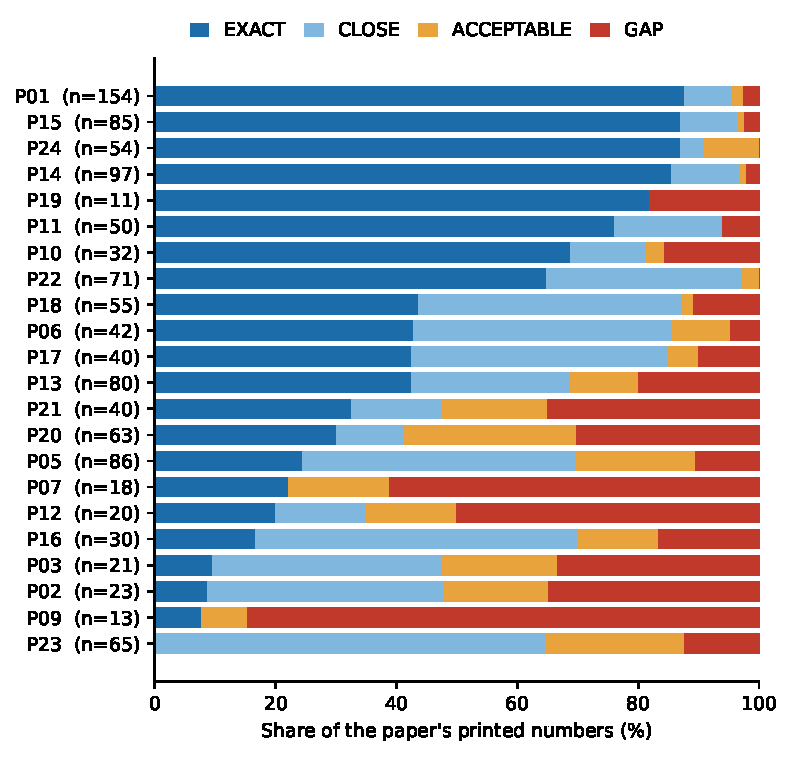
\includegraphics[width=0.62\textwidth]{figures/fig2_audit_overview.pdf}
\caption{Outcome of the audit of 21 published NHTS studies (P01-P23; listed in the repository, first-audit scripts). Bars show the share of each study's printed numbers that pynhts reproduces exactly, closely (2\,\%), acceptably (5\,\%) or not.}
\label{fig:audit}
\end{figure}

The exercise produced 32 recovered conventions, written down with their evidence, and several of them change published numbers. A re-check of one study \cite{lidbe} with the crosswalks and the study module illustrates this: 262 of 280 cells of its Tables 3 and 4 are reproduced exactly (Fig.~\ref{fig:lidbe}). The percentages in its Table 3 use the trips of persons with a valid answer as the base (Example 2); its weekend is Saturday and Sunday of the travel-day variable, whereas the NHTS weekend flag also contains part of Friday and gives values 5 to 8\,\% higher; trip duration is the calculated minutes variable; the six items on how the condition changes travel are reproduced exactly (72 of 72 cells) through the condition-effect crosswalk; and its race groups follow a rule in which Hispanic origin overrides only the White, Black and Asian groups, which is not what a combined race-and-ethnicity variable does. In another study \cite{yang} the sample of 130,222 persons is reproduced exactly as a Study, and its race variable is the household respondent's single race code; mapping it through the combined variable would give a different sample (133,538 persons). These findings became package features (crosswalks, caps, warnings) or documentation.

\begin{figure}[!ht]
\centering
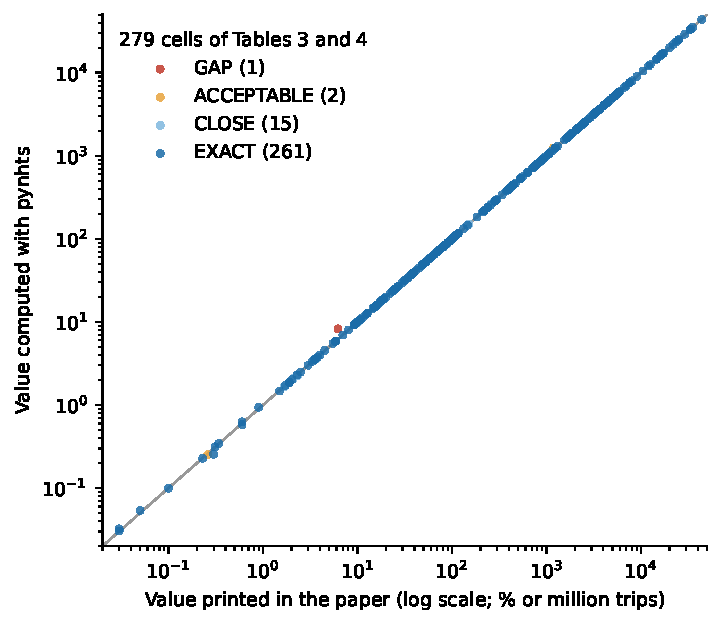
\includegraphics[width=0.62\textwidth]{figures/fig3_agreement_lidbe.pdf}
\caption{Values printed in Tables 3 and 4 of Lidbe et al. \cite{lidbe} against the values computed with pynhts (279 cells with a positive value; one printed zero is not shown). The diagonal is exact agreement.}
\label{fig:lidbe}
\end{figure}

\textbf{New research questions and changed practice}\\[2pt]

Design-correct uncertainty for every wave, guarded comparisons across waves, and sample-flow tables make it cheaper to ask questions that depend on trends and on subpopulations, and to report them so that others can repeat them. The study module is meant to change the daily practice of analysts by making the sample rules and the missing-value policy part of the code. We have not measured any change in practice yet.

\textbf{Extent of use}\\[2pt]

The first version was released on PyPI in October 2026 and the package has had 13 releases in total; version 0.8.1 is archived on Zenodo \cite{software}. The package has no known external users, no publication has used it, and it has no commercial use. PyPI records downloads, but they include automated mirrors, so we do not report them as users. The evidence of impact is therefore the validation and the audit, which can be repeated by anyone with the public files, and the intended use is by researchers who analyse the NHTS and by those who review such analyses.

\item \textbf{Conclusions}\label{sec:conclusions}\\

pynhts gives researchers typed, survey-weighted access to the four NHTS waves with the variance method of each wave, crosswalks that are checked against the data, and a way to state the sample and the missing-value policy as code. Its validation against official figures and published studies shows both that it reproduces most numbers and that the remaining differences usually come from rules that publications do not state.

Limitations are clear. The package is at an alpha stage and its interface may change. It handles the public-use files only; variables that need the restricted files (for example census-tract identifiers) are out of reach. It does not fit models, so standard errors of regression coefficients, which need the weights to be refitted for each replicate, are not yet provided. National weights of the 2001 national sample are not available. The replicate-weight archives of 2001 and 2009 are large. Next steps are variance estimates for model coefficients, more crosswalks, and a repeated audit as new studies appear.

\end{enumerate}

\section*{Acknowledgements}

The NHTS is conducted by the US Department of Transportation, Federal Highway Administration, and distributed by Oak Ridge National Laboratory. The package does not redistribute the survey data.

\section*{Declaration of generative AI and AI-assisted technologies in the manuscript preparation process}

During the preparation of this work the authors used Claude (Anthropic) as an assistant for software design, writing and running code and tests, checking the code against the official documents and data, literature screening, and drafting and editing the text. After using this tool, the authors reviewed, verified and edited the material (code, results, references and text) and take full responsibility for the content of the publication. Numbers in the text are taken by code from the result files of the repository, and the references were checked against a bibliographic database.

\section*{CRediT authorship contribution statement}

Seyed Saber Naseralavi: Conceptualization, Data curation, Formal analysis, Investigation, Methodology, Project administration, Resources, Software, Validation, Visualization, Writing - original draft, Writing - review and editing. Akram Mazaheri: [[AUTHOR-TODO: CRediT roles of A. Mazaheri; not stated by the authors]]

\section*{Funding}

This research did not receive any specific grant from funding agencies in the public, commercial, or not-for-profit sectors.

\section*{Declaration of competing interest}

The authors declare that they have no known competing financial interests or personal relationships that could have appeared to influence the work reported in this paper.

\section*{Data availability}

The software is available at https://github.com/sabernaseralavi-60/pynhts (archived at Zenodo, DOI 10.5281/zenodo.23575312). The NHTS public-use data are distributed by Oak Ridge National Laboratory (https://nhts.ornl.gov); pynhts downloads them from there and does not redistribute them.

\begin{thebibliography}{00}

\bibitem{mcguckin} McGuckin N, Fucci A. Summary of travel trends: 2017 National Household Travel Survey. Report FHWA-PL-18-019. Washington (DC): US Department of Transportation, Federal Highway Administration; 2018. \url{https://nhts.ornl.gov/assets/2017_nhts_summary_travel_trends.pdf} [accessed 22 October 2026].

\bibitem{labban} Labban M, Chen CR, Frego N, Nguyen DD, Lipsitz SR, Reich AJ, et al. Disparities in travel-related barriers to accessing health care from the 2017 National Household Travel Survey. JAMA Netw Open 2023;6:e2325291. \url{https://doi.org/10.1001/jamanetworkopen.2023.25291}.

\bibitem{buehler} Buehler R, Pucher J, Wittwer R, Gerike R. Travel behavior of older adults in the USA, 2001-2017. Travel Behav Soc 2024;36:100783. \url{https://doi.org/10.1016/j.tbs.2024.100783}.

\bibitem{akinlotan} Akinlotan M, Khodakarami N, Primm K, Bolin J, Ferdinand AO. Travel for medical or dental care by race/ethnicity and rurality in the U.S.: findings from the 2001, 2009 and 2017 National Household Travel Surveys. Prev Med Rep 2023;35:102297. \url{https://doi.org/10.1016/j.pmedr.2023.102297}.

\bibitem{lidbe} Lidbe A, Adanu EK, Penmetsa P, Jones S. Changes in the travel patterns of older Americans with medical conditions: a comparison of 2001 and 2017 NHTS data. Transp Res Interdiscip Perspect 2021;11:100463. \url{https://doi.org/10.1016/j.trip.2021.100463}.

\bibitem{conway} Conway MW, Salon D, King DA. Trends in taxi use and the advent of ridehailing, 1995-2017: evidence from the US National Household Travel Survey. Urban Sci 2018;2:79. \url{https://doi.org/10.3390/urbansci2030079}.

\bibitem{rafiq} Rafiq R, McNally MG. An exploratory analysis of alternative travel behaviors of ride-hailing users. Transportation 2023;50:571-605. \url{https://doi.org/10.1007/s11116-021-10254-9}.

\bibitem{zhang} Zhang Y, Zhang Y. Examining the relationship between household vehicle ownership and ridesharing behaviors in the United States. Sustainability 2018;10:2720. \url{https://doi.org/10.3390/su10082720}.

\bibitem{li} Li X, Liu C, Jia J. Ownership and usage analysis of alternative fuel vehicles in the United States with the 2017 National Household Travel Survey data. Sustainability 2019;11:2262. \url{https://doi.org/10.3390/su11082262}.

\bibitem{alberini} Alberini A, Teja Burra L, Cirillo C, Shen C. Counting vehicle miles traveled: what can we learn from the NHTS? Transp Res Part D Transp Environ 2021;98:102984. \url{https://doi.org/10.1016/j.trd.2021.102984}.

\bibitem{wu} Wu X, MacKenzie D. Assessing the VMT effect of ridesourcing services in the US. Transp Res Part D Transp Environ 2021;94:102816. \url{https://doi.org/10.1016/j.trd.2021.102816}.

\bibitem{yang} Yang Y, Diez Roux AV, Bingham CR. Variability and seasonality of active transportation in USA: evidence from the 2001 NHTS. Int J Behav Nutr Phys Act 2011;8:96. \url{https://doi.org/10.1186/1479-5868-8-96}.

\bibitem{zhou} Zhou Y, Wang X(C). Explore the relationship between online shopping and shopping trips: an analysis with the 2009 NHTS data. Transp Res Part A Policy Pract 2014;70:1-9. \url{https://doi.org/10.1016/j.tra.2014.09.014}.

\bibitem{wang} Wang X, Shaw FA, Mokhtarian PL, Watkins KE. Response willingness in consecutive travel surveys: an investigation based on the National Household Travel Survey using a sample selection model. Transportation 2023;50:2339-73. \url{https://doi.org/10.1007/s11116-022-10312-w}.

\bibitem{yoshikawa} Yoshikawa S, Maruyama T. Proxy responses contain more rounded trip departure/arrival times: evidence from the 2017 US National Household Travel Survey. J JSCE 2023;11. \url{https://doi.org/10.2208/journalofjsce.23-00137}.

\bibitem{esekhaigbe} Esekhaigbe EO, Bills TS, Broaddus A. Group representation of vulnerable travelers in household travel surveys: an assessment of 43 U.S. surveys. Transportation 2026. \url{https://doi.org/10.1007/s11116-026-10795-x}.

\bibitem{zheng} Zheng Z. Reasons, challenges, and some tools for doing reproducible transportation research. Commun Transp Res 2021;1:100004. \url{https://doi.org/10.1016/j.commtr.2021.100004}.

\bibitem{wood} Wood J, van Schalkwyk I. Reproducibility in transportation research: importance, best practices, and dealing with protected and sensitive data. J Transp Technol 2025;15:179-202. \url{https://doi.org/10.4236/jtts.2025.151010}.

\bibitem{horl} H\"orl S, Bala\'c M. Synthetic population and travel demand for Paris and \^Ile-de-France based on open and publicly available data. Transp Res Part C Emerg Technol 2021;130:103291. \url{https://doi.org/10.1016/j.trc.2021.103291}.

\bibitem{lamprecht} Lamprecht AL, Garcia L, Kuzak M, Martinez C, Arcila R, Martin Del Pico E, et al. Towards FAIR principles for research software. Data Sci 2020;3:37-59. \url{https://doi.org/10.3233/ds-190026}.

\bibitem{barker} Barker M, Chue Hong NP, Katz DS, Lamprecht AL, Martinez-Ortiz C, Psomopoulos F, et al. Introducing the FAIR principles for research software. Sci Data 2022;9:622. \url{https://doi.org/10.1038/s41597-022-01710-x}.

\bibitem{smith} Smith AM, Katz DS, Niemeyer KE; FORCE11 Software Citation Working Group. Software citation principles. PeerJ Comput Sci 2016;2:e86. \url{https://doi.org/10.7717/peerj-cs.86}.

\bibitem{summarize} Westat Transportation. summarizeNHTS: R package for summarizing NHTS data [software]. \url{https://github.com/Westat-Transportation/summarizeNHTS} [accessed 22 October 2026].

\bibitem{lumley} Lumley T. Analysis of complex survey samples. J Stat Softw 2004;9(8). \url{https://doi.org/10.18637/jss.v009.i08}.

\bibitem{samplics} Diallo M. samplics: a Python package for selecting, weighting and analyzing data from complex sampling designs. J Open Source Softw 2021;6:3376. \url{https://doi.org/10.21105/joss.03376}.

\bibitem{wolter} Wolter KM. Introduction to variance estimation. 2nd ed. New York: Springer; 2007. \url{https://doi.org/10.1007/978-0-387-35099-8}.

\bibitem{weighting} Roth SB, DeMatteis J, Dai Y. 2017 NHTS weighting report. Westat, prepared for the Federal Highway Administration; 2017. \url{https://nhts.ornl.gov/assets/2017\%20NHTS\%20Weighting\%20Report.pdf} [accessed 22 October 2026].

\bibitem{software} Naseralavi SS. pynhts: survey-weight-aware access to US National Household Travel Survey microdata. Version 0.8.1 [software]. Zenodo; 2026 Oct 22. \url{https://doi.org/10.5281/zenodo.23575312}.

\end{thebibliography}

\section*{Current executable software version}

Not applicable: pynhts is a Python library without a separate executable. Install version 0.8.1 with pip install pynhts==0.8.1.

\end{document}
